\documentclass[12pt, a4paper]{article}
\usepackage[a4paper, includeheadfoot, mag=1000, left=2cm, right=1.5cm, top=1.5cm, bottom=1.5cm, headsep=0.8cm, footskip=0.8cm]{geometry}
% Fonts
\usepackage{fontspec, unicode-math}
\setmainfont[Ligatures=TeX]{CMU Serif}
\setmonofont{CMU Typewriter Text}
\usepackage[english, russian]{babel}
% Indent first paragraph
\usepackage{indentfirst}
\setlength{\parskip}{5pt}
% Diagrams
\usepackage{graphicx}
\usepackage{float}
% Page headings
\usepackage{fancyhdr}
\pagestyle{fancy}
\renewcommand{\headrulewidth}{0pt}
\setlength{\headheight}{16pt}
%\newfontfamily\namefont[Scale=1.2]{Gloria Hallelujah}
\fancyhead{}

\usepackage{amsmath}

\graphicspath{ {./images/} }

\usepackage{listings}
\lstdefinestyle{lablisting}{
  basicstyle=\scriptsize\ttfamily,
  numbers=left,
  stepnumber=1,
  otherkeywords={EOF, O\_RDONLY, STDIN\_FILENO, STDOUT\_FILENO, STDERR\_FILENO},
  numbersep=10pt,
  showspaces=false,
  showstringspaces=false
}

\newcommand{\specialcell}[2][l]{%
  \begin{tabular}[#1]{@{}l@{}}#2\end{tabular}}

\begin{document}

% Title page
\begin{titlepage}
\begin{center}

\textsc{Федеральное государственное автономное образовательное учреждение высшего\\
образования "Национальный исследовательский университет ИТМО"}
\vfill
\textbf{Лабораторная работа №1\\[4mm]
по дисципение "Информационная безопасность"\\[4mm]
Основы шифрования данных\\[4mm]
}
\textit{Вариант 10\\[20mm]}
\begin{flushright}
Выполнил: студент Саржевский И.А.
\\[2mm]Группа: P3402\\[4mm]
Преподаватель: к.т.н., доцент\\
Маркина Т.А.
\end{flushright}
\vfill
г. Санкт-Петербург\\[2mm]
2021 г.

\end{center}
\end{titlepage}

\begin{huge}Лабораторная работа №1\end{huge}\\[4mm]
\begin{Large}Основы шифрования данных\end{Large}\\

\section*{Цель работы}

Изучение основных принципов шифрования информации, знакомство
с широко известными алгоритмами шифрования, приобретение навыков
их программной реализации.

\section*{Задание}

\textbf{Вариант: 10}. Реализовать в программе шифрование и дешифрацию
содержимого файла по методу Цезаря. Провести частотный анализ
зашифрованного файла, осуществляя проверку по файлу с набором
ключевых слов.

Метод Цезаря заключается в том, что весь алфавит циклически сдвигается
на заданное количество шагов направо или налево, и исходное сообщение
записывается при помощи алфавита, индексы которого сдвинуты. Для того,
чтобы раскодировать сообщение необходимо провести обратную операцию -
сдвиг индексов алфавита в обратном направлении на такое же количество
шагов.

Помимо реализации медота Цезаря, в задании предлагается реализовать
расшифровку закодированного файла используя частотный анализ. Для этого
воспользуемся статистической информацией о распределении частоты
использования букв английского алфавита и попробуем сопоставить эти
данные с частотой использования букв в зашифрованном сообщении,
таким образом восстановив изначальные символы.

\begin{figure}[H]
  \centering
  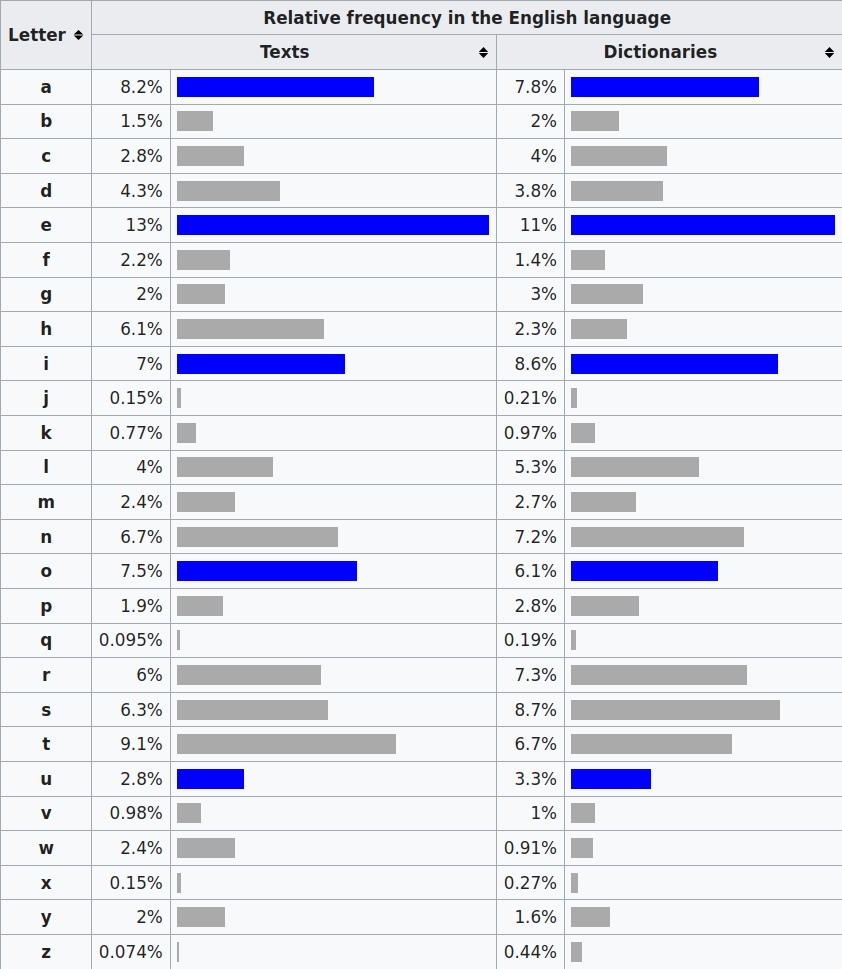
\includegraphics[scale = 0.5]{freq}
  \caption{Относительная частота встречаемости в текстах букв английского алфавита}
\end{figure}

\newpage
\section*{Листинг разработанной программы}

\subsubsection*{main.rs}

\lstinputlisting[style=lablisting]{../src/main.rs}

\subsubsection*{alphabet.rs}

\lstinputlisting[style=lablisting]{../src/alphabet.rs}

\subsubsection*{caesar.rs}

\lstinputlisting[style=lablisting]{../src/caesar.rs}

\subsubsection*{freq\_analysis.rs}

\lstinputlisting[style=lablisting]{../src/freq_analysis.rs}

\section*{Результаты работы программы}

\begin{figure}[h]
    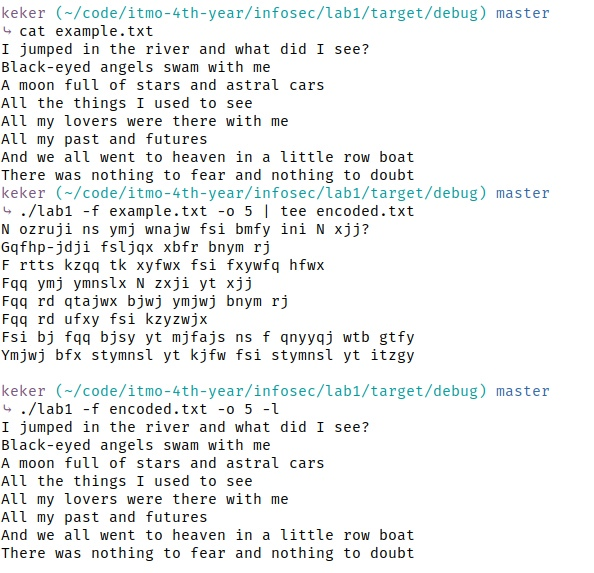
\includegraphics[scale = 0.55]{res1}
    \caption{Результат работы программы (обычный режим)}
    \centering
\end{figure}

\begin{figure}[H]
  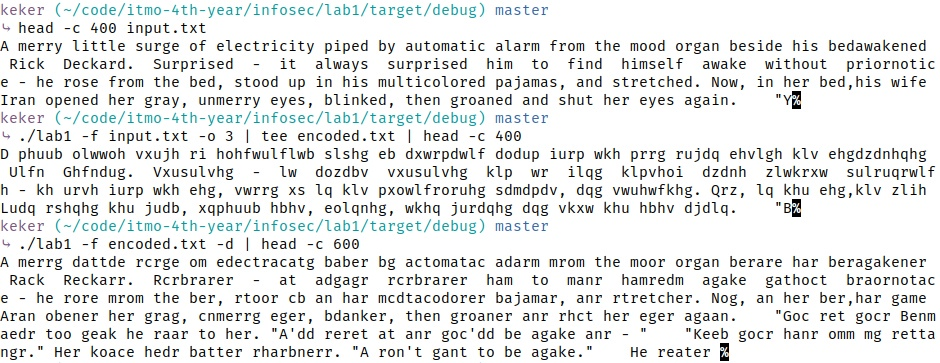
\includegraphics[scale = 0.55]{res2}
  \caption{Результат работы программы (частотный анализ)}
  \centering
\end{figure}

\section*{Вывод}

В результате выполнения данной лабораторной работы был имплементирован
шифр Цезаря для шифрования файла и метод частотного анализа для его
дешифровки. Нужно отметить, что полностью восстановить исходный текст
не удалось, так как дешифрующий метод основан на статистических данных.
Тем не менее, некоторые ключевые слова удалось распознать - organ, he,
her, to, be. В случае с шифром Цезаря этого более чем достаточно, чтобы
определить смещение и раскодировать все сообщение.

\end{document}
